\chapter{Parallelization}
In the experiments described in this study, the bulk of processing time is spent evaluating the genomes using roborobo.
The genome evaluations are independent of each other, and is therefore a good candidate for parallelization.
With a great number of global variables, the roborobo framework itself is not easily parallelized.
The solution was to use \emph{Message passing interface(MPI)} to run multiple cooperating roborobo processes. 

The parallelization is done by letting one root process take responsibility for running the evolutionary algorithm, with multiple slave processes for evaluating the genomes.

\begin{figure}[H]
	\centering
	\begin{subfigure}[t]{0.45\textwidth}
		\centering
		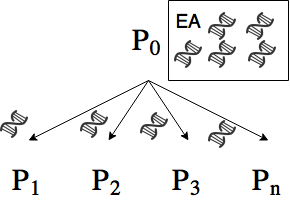
\includegraphics[scale=0.5]{chapters/res/mpi-distribute.png}
		\caption{Distributing the genomes from the root process to the slave processes for evaluation.}
		\label{fig:distribute-genomes}
	\end{subfigure}
	\begin{subfigure}[t]{0.45\textwidth}
		\centering
		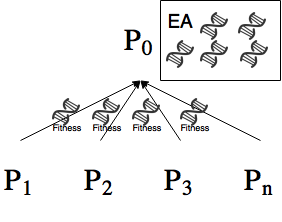
\includegraphics[scale=0.5]{chapters/res/mpi-gather.png}
		\caption{Gathering the evaluated genomes from the slave processes.}
		\label{fig:gather-genomes}
	\end{subfigure}
	\caption{Distributing and gathering genomes.}
\end{figure}
At the beginning of each generation the root process generates the new genomes from the evolutionary algorithm.
The new genomes are then distributed evenly to each process, see figure \ref{fig:distribute-genomes}.
Once all the genomes are evaluated, the root process gathers the evaluated genomes from the slave processes, see figure \ref{fig:gather-genomes}.
The evaluated genomes are then used by the evolutionary algorithm to create the next generation.
This process is repeated until the target fitness is reached or a processing threshold is met. 

\chapter{Configuration \&  Code}

The project code and system configuration can be found at \url{https://github.com/christjt/ntnu-project-2016}




